\documentclass{ximera}

\author{Anna Davis \and Paul Zachlin} \title{Composition and Inverses of Linear Transformations} \license{CC-BY 4.0}

\renewcommand{\vec}[1]{{\bf #1}}
\newcommand{\RR}{\mathbb{R}}
\newcommand{\dfn}{\textit}
\newcommand{\dotp}{\cdot}
\newcommand{\id}{\text{id}}

\newtheorem{general}{Generalization}
\newtheorem{initprob}{Exploration Problem}
\usepackage{tikz-cd}
\usetikzlibrary{shapes.geometric}
\usetikzlibrary{arrows}
\pgfplotsset{compat=1.14}



\begin{document}
\begin{abstract}
  We define composition of linear transformations, inverse of a linear transformation, and discuss existence and uniqueness of inverses.
\end{abstract}
\maketitle

%Note to Student:  In this module we will often use $U$, $V$ and $W$ to denote the domain and codomain of linear transformations.  If you are familiar with abstract vector spaces, you can regard $U$, $V$ and $W$ as finite-dimensional vector spaces, otherwise you may think of $U$, $V$ and $W$ as subspaces of $\RR^n$. 

%Recall that a transformation $T:\mathbb{R}^n\rightarrow \mathbb{R}^m$ is called a {\it linear transformation} if the following are true for all vectors ${\bf u}$ and ${\bf v}$ in $\mathbb{R}^n$, and scalars $k$.
%\begin{equation*}
%T(k{\bf u})= kT({\bf u})
%\end{equation*}
%\begin{equation*}
%T({\bf u}+{\bf v})= T({\bf u})+T({\bf v})
%\end{equation*}

%We generalize this definition as follows.

%\begin{definition}\label{def:lintransgeneral}
%A transformation $T:V\rightarrow W$ is called a {\it linear transformation} if the following are true for all vectors ${\bf u}$ and ${\bf v}$ in $V$, and scalars $k$.
%\begin{equation*}
%T(k{\bf u})= kT({\bf u})
%\end{equation*}
%\begin{equation*}
%T({\bf u}+{\bf v})= T({\bf u})+T({\bf v})
%\end{equation*}
%\end{definition}

\section*{Composition of Linear Transformations}

\subsection*{Definition and Properties}
\begin{definition} Let $U$, $V$ and $W$ be vector spaces, and let $T:U\rightarrow V$ and $S:V\rightarrow W$ be linear transformations.  The composition of $S$ and $T$ is the transformation $S\circ T:U\rightarrow W$ given by
$$(S\circ T)(\vec{u})=S(T(\vec{u}))$$
\end{definition}

\begin{example}\label{ex:transcomp} Define $$T:\RR^2\rightarrow \RR^2 \quad\text{by}\quad T\left(\begin{bmatrix}u_1\\u_2\end{bmatrix}\right)=\begin{bmatrix}u_1+u_2\\3u_1+3u_2\end{bmatrix}$$

$$S:\RR^2\rightarrow \RR^2 \quad\text{by}\quad S\left(\begin{bmatrix}v_1\\v_2\end{bmatrix}\right)=\begin{bmatrix}3v_1-v_2\\-3v_1+v_2\end{bmatrix}$$
Examine the effect of $S\circ T$ on vectors of $\RR^2$.
\begin{explanation}
From the computational standpoint, the situation is simple.
\begin{align*}
(S\circ T)\left(\begin{bmatrix}u_1\\u_2\end{bmatrix}\right)&=S\left(T\left(\begin{bmatrix}u_1\\u_2\end{bmatrix}\right)\right)=S\left(\begin{bmatrix}u_1+u_2\\3u_1+3u_2\end{bmatrix}\right)\\
&=\begin{bmatrix}3(u_1+u_2)-(3u_1+3u_2)\\-3(u_1+u_2)+(3u_1+3u_2)\end{bmatrix}\\
&=\vec{0}
\end{align*}
This means that $S\circ T$ maps all vectors of $\RR^2$ to $\vec{0}$.  

In addition to the computational approach, it is also useful to visualize what happens geometrically.

First, observe that $T\left(\begin{bmatrix}u_1\\u_2\end{bmatrix}\right)=\begin{bmatrix}u_1+u_2\\3u_1+3u_2\end{bmatrix}=(u_1+u_2)\begin{bmatrix}1\\3\end{bmatrix}$  So, the image of any vector of $\RR^2$ under $T$ lies on the line determined by the vector $\begin{bmatrix}1\\3\end{bmatrix}$.  

Even though $S$ is defined on all of $\RR^2$, we are only interested in the action of $S$ on vectors along the line determined by $\begin{bmatrix}1\\3\end{bmatrix}$.  Our computations showed that all such vectors map to $\vec{0}$.

The actions of individual transformations, as well as the composite transformation are shown below.

\begin{image}[3.5in]\label{fig:actionofst} 
\centering
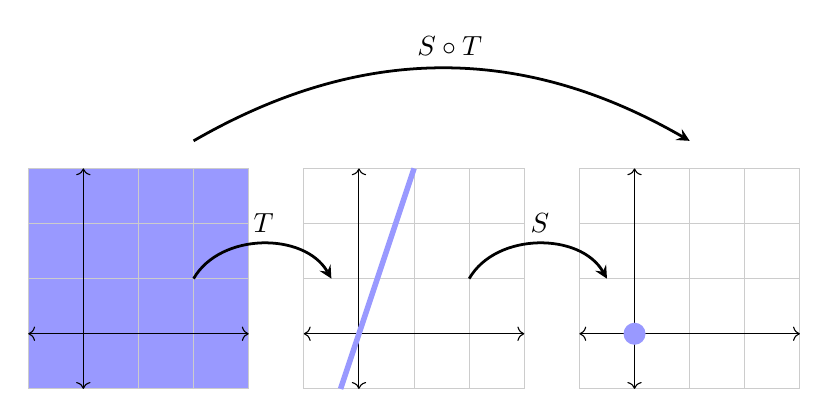
\begin{tikzpicture}[scale=.7]

\fill[blue!40] (-1,-1) rectangle (3,3);
\draw[thin,gray!40] (-1,-1) grid (3,3);
  \draw[<->] (-1,0)--(3,0);
  \draw[<->] (0,-1)--(0,3);

  \draw[thin,gray!40] (4,-1) grid (8,3);
  \draw[<->] (4,0)--(8,0);
  \draw[<->] (5,-1)--(5,3);
  \draw[line width=2pt,blue!40](14/3,-1)--(6,3) node[anchor=south west]{};
  
  \draw[thin,gray!40] (9,-1) grid (13,3);
  \draw[<->] (9,0)--(13,0);
  \draw[<->] (10,-1)--(10,3);
  %\draw[line width=2pt,red,-stealth](0,0)--(-1,-1) node[anchor=north east]{$-\vec{u}$};
  \fill[blue!40!white] (10,0) circle (0.2cm);
  \draw [->,line width=1pt,-stealth]  (2,1)to[out=60, in=120](4.5, 1)node[above=7mm, left=6mm]{$T$};
\draw [->,line width=1pt,-stealth] (7,1)to[out=60, in=120](9.5, 1)node[above=7mm, left=6mm]{$S$};
\draw [->,line width=1pt,-stealth] (2,3.5)to[out=30, in=150](11, 3.5)node[above=12mm, left=25mm]{$S\circ T$};
\end{tikzpicture}
%\caption{The action of $T$, $S$ and $S\circ T$.}
  
\end{image}

\end{explanation}
\end{example}

\begin{theorem}\label{th:complinear}
The composition of two linear transformations is linear.
\end{theorem}
\begin{proof}
Let $T:U\rightarrow V$ and $S:V\rightarrow W$ be linear transformations. We will show that $S\circ T$ is linear.  For all vectors $\vec{u}_1$ and $\vec{u}_2$ of $U$ and scalars $a$ and $b$ we have:
\begin{align*}
(S\circ T)(a\vec{u}_1+b\vec{u}_2)&=S(T(a\vec{u}_1+b\vec{u}_2))\\
&=S(aT(\vec{u}_1)+bT(\vec{u}_2))\\
&=aS(T(\vec{u}_1))+bS(T(\vec{u}_2))\\
&=a(S\circ T)(\vec{u}_1)+b(S\circ T)(\vec{u}_2)
\end{align*}
\end{proof}

\begin{theorem}Composition of linear transformations is associative.  In other words, for linear transformations  $T$, $S$ and $R$

\begin{center}
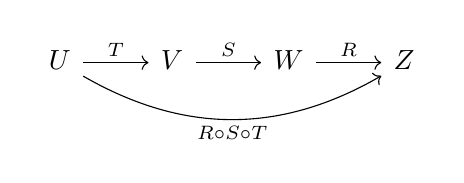
\begin{tikzpicture}
\node{
\begin{tikzcd}
U\rar{T}\arrow[black, bend right]{rrr}[black,swap]{R\circ S\circ T}  & V \rar{S}  & W \rar{R} & Z
\end{tikzcd}
};
\end{tikzpicture}
\end{center}
We have $(R\circ S)\circ T=R\circ (S\circ T)$.
\end{theorem}
\begin{proof} For all $\vec{u}$ in $U$ we have:
\begin{align*}
((R\circ S)\circ T)(\vec{u})&=(R\circ S)(T(\vec{u}))=R(S(T(\vec{u})))\\
&=R((S\circ T)(\vec{u}))=(R\circ (S\circ T))(\vec{u})
\end{align*}
\end{proof}

\subsection*{Composition and Matrix Multiplication}

In this section we will consider linear transformations of $\RR^n$ and their standard matrices.  

\begin{theorem}
Let $T:\RR^n\rightarrow \RR^m$ and $S:\RR^m\rightarrow \RR^p$ be linear transformations with standard matrices $M_T$ and $M_S$, respectively.  Then the composite transformation $S\circ T:\RR^n\rightarrow \RR^p$ has a standard matrix given by the product $M_SM_T$.
\end{theorem}
\begin{proof}
For all $\vec{v}$ in $\RR^n$ we have:
$$(S\circ T)(\vec{v})=S(T(\vec{v}))=S(M_T\vec{v})=M_S(M_T\vec{v})=(M_SM_T)\vec{v}$$
\end{proof}

\begin{example}
In Example \ref{ex:transcomp}, we discussed a composite transformation $S\circ T:\RR^2\rightarrow \RR^2$
given by:
$$T\left(\begin{bmatrix}u_1\\u_2\end{bmatrix}\right)=\begin{bmatrix}u_1+u_2\\3u_1+3u_2\end{bmatrix}\quad \text{and} \quad
S\left(\begin{bmatrix}v_1\\v_2\end{bmatrix}\right)=\begin{bmatrix}3v_1-v_2\\-3v_1+v_2\end{bmatrix}$$
Express $S\circ T$ as a matrix transformation.
\begin{explanation}
The standard matrix for $T:\RR^2\rightarrow \RR^2$ is $$\begin{bmatrix}1&1\\3&3\end{bmatrix}$$ and the standard matrix for $S:\RR^2\rightarrow \RR^2$ is $$\begin{bmatrix}3&-1\\-3&1\end{bmatrix}$$
The standard matrix for $S\circ T$ is the product
$$\begin{bmatrix}3&-1\\-3&1\end{bmatrix}\begin{bmatrix}1&1\\3&3\end{bmatrix}=\begin{bmatrix}0&0\\0&0\end{bmatrix}$$
\end{explanation}
\end{example}

We conclude this section by revisiting the associative property of matrix multiplication.  At the time matrix multiplication was introduced, you might have found it cumbersome to prove that for appropriately sized matrices $A$, $B$ and $C$, we have $(AB)C=A(BC)$ (See Theorem \ref{th:propertiesofmatrixmultiplication}).  We are now in a position to prove this result with ease.  

Every matrix induces a linear transformation.  The product of two matrices can be interpreted as a composition of transformations.  Since transformation composition is associative, so is matrix multiplication. We formalize this observation as a theorem.

\begin{theorem}[Associativity of Matrix Multiplication] \label{th:associativematrixmult}  Let $A$, $B$ and $C$ be matrices of appropriate dimensions so that the product $(AB)C$ is defined.  Then
$$ABC=(AB)C=A(BC)$$
\end{theorem}

\section*{Inverses of Linear Transformations}

\begin{initprob}\label{ep:inverse} Define a linear transformation $T:\RR^2\rightarrow \RR^2$ by $T(\vec{v})=2\vec{v}$.  In other words, $T$ doubles every vector in $\RR^2$.  Now define $S:\RR^2\rightarrow \RR^2$ by $S(\vec{v})=\frac{1}{2}\vec{v}$.  What happens when we compose these two transformations?
$$(S\circ T)(\vec{v})=S(T(\vec{v}))=S(2\vec{v})=\left(\frac{1}{2}\right)(2)\vec{v}=\vec{v}$$
$$(T\circ S)(\vec{v})=T(S(\vec{v}))=T(\frac{1}{2}\vec{v})=(2)\left(\frac{1}{2}\right)\vec{v}=\vec{v}$$
Both composite transformations return the original vector $\vec{v}$.  In other words, $S\circ T=\id_{\RR^2}$ and $T\circ S=\id_{\RR^2}$.  We say that $S$ is an \dfn{inverse} of $T$, and $T$ is an inverse of $S$.
\end{initprob}

% \subsection*{Definition of an Inverse Transformation}
% {\color{green} Paul, In Definition 2, do we need to require that T is linear? If we don't, we would have a more general definition of an inverse.  Later we have a theorem that says that an inverse of a linear transformation is linear.}
\begin{definition}\label{def:inverse} Let $V$ and $W$ be vector spaces, and let $T:V\rightarrow W$ be a linear transformation.  A transformation $S:W\rightarrow V$ such that $S\circ T=\id_V$ and $T\circ S=\id_W$ is called an inverse of $T$. If $T$ has an inverse, $T$ is called invertible.
\end{definition}

\begin{example}\label{ex:inverseverify} Let $T:\RR^2\rightarrow \RR^2$ be a transformation defined by $T\left(\begin{bmatrix}x\\y\end{bmatrix}\right)=\begin{bmatrix}x+y\\x-y\end{bmatrix}$. (How would you verify that $T$ is linear?)  Show that $S:\RR^2\rightarrow \RR^2$ given by $S\left(\begin{bmatrix}x\\y\end{bmatrix}\right)=\begin{bmatrix}0.5x+0.5y\\0.5x-0.5y\end{bmatrix}$ is an inverse of $T$.
\begin{explanation}
We will show that $S\circ T=\id_{\RR^2}$.  
\begin{align*}
(S\circ T)\left(\begin{bmatrix}x\\y\end{bmatrix}\right)&=S\left(T\left(\begin{bmatrix}x\\y\end{bmatrix}\right)\right)=S\left(\begin{bmatrix}x+y\\x-y\end{bmatrix}\right)\\
&=\begin{bmatrix}0.5(x+y)+0.5(x-y)\\0.5(x+y)-0.5(x-y)\end{bmatrix}
=\begin{bmatrix}x\\y\end{bmatrix}
\end{align*}
We leave it to the reader to verify that $T\circ S=\id_{\RR^2}$.

\end{explanation}
\end{example}

\subsection*{Linearity of Inverses of Linear Transformations}

Definition \ref{def:inverse} does not specifically require an inverse $S$ of a linear transformation $T$ to be linear.  This is because the requirement that $S\circ T=\id_V$ and $T\circ S=\id_W$ is sufficient to guarantee that $S$ is linear.  

\begin{theorem}\label{th:inverseislinear} Suppose $T:V\rightarrow W$ is an invertible linear transformation.  Let $S$ be an inverse of $T$.  Then $S$ is  linear.
\end{theorem}

\begin{proof} The proof of this result is left to the reader. (See Practice Problem \ref{prob:inverseislinear})
%Let $\vec{w}_1$ and $\vec{w}_2$ be vectors in $W$ such that $\vec{w}_1=T(\vec{v}_1)$ and $T(\vec{w}_2)=\vec{v}_2$ for some $\vec{v}_1$ and $\vec{v}_2$ in $V$. Let $k_1$ and $k_2$ be scalars.
%\begin{align*}
%S(k_1\vec{w}_1+k_2\vec{w}_2)&=S(k_1T(\vec{v}_1)+k_2T(\vec{v}_2))\\
%&=S(T(k_1\vec{v}_1+k_2\vec{v}_2))\\
%&=(S\circ T)(k_1\vec{v}_1+k_2\vec{v}_2)\\
%&=k_1\vec{v}_1+k_2\vec{v}_2\\
%&=k_1S(\vec{w}_1)+k_2S(\vec{w}_2)
%\end{align*}
%Therefore $S$ is linear.
\end{proof}


\subsection*{Linear Transformations of $\RR^n$ and the Standard Matrix of the Inverse Transformation}

Every linear transformation $T:\RR^n\rightarrow\RR^m$ is a matrix transformation. (See Theorem \ref{matlin})  If $T$ has an inverse $S$, then $S$ is also a matrix transformation.  Let  $M_T$ and $M_S$ denote the standard matrices of $T$ and $S$, respectively.  We see that $S\circ T=\id_{\RR^n}$ and $T\circ S=\id_{\RR^m}$ if and only if $M_SM_T=I_{n}$ and $M_TM_S=I_{m}$.  In other words, $T$ and $S$ are inverse transformations if and only if $M_T$ and $M_S$ are matrix inverses.

Note that if $S$ is an inverse of $T$, then $M_T$ and $M_S$ are square matrices, and $n=m$. 

\begin{theorem}\label{th:existunique} Let $T:\RR^n\rightarrow \RR^n$ be a linear transformation, and let $M$ be the standard matrix of $T$.
  \begin{enumerate}
  \item \label{item:exists} {\bf Existence of Inverses.}  $T$ is invertible if and only if $M$ is invertible.  If $T$ is invertible, then the inverse is induced by $M^{-1}$.
  \item \label{item:unique}{\bf Uniqueness of Inverses.}  If $S$ is an inverse of $T$, then $S$ is unique.
  \end{enumerate}
\end{theorem}
\begin{proof}
Part \ref{item:exists} follows directly from the preceding discussion.  Part \ref{item:unique} follows from uniqueness of matrix inverses. (Theorem \ref{th:matinverseunique})
\end{proof}

%Theorem \ref{th:existunique} may be a little misleading because it appears to imply that the question of existence of an inverse can be settled entirely by finding (or not finding) the inverse of the standard matrix of a linear transformation.  So, why look at anything else?  Consider the following set up.

% {\color{green} Paul, please check the blue paragraph.  The old paragraph is commented out, if you'd like to compare.}

Please note that Theorem \ref{th:existunique} is only applicable in the context of linear transformations of $\RR^n$ and their standard matrices.  The following example provides us with motivation to investigate inverses further, which we will do in another module.

\begin{initprob}\label{init:subtosub}
Let $$V=\text{span}\left(\begin{bmatrix}1\\0\\0\end{bmatrix}, \begin{bmatrix}1\\1\\1\end{bmatrix}\right)$$
Define a linear transformation $$T:V\rightarrow \RR^2$$
by $$T\left(\begin{bmatrix}1\\0\\0\end{bmatrix}\right)=\begin{bmatrix}1\\1\end{bmatrix}\quad \text{and} \quad T\left(\begin{bmatrix}1\\1\\1\end{bmatrix}\right)=\begin{bmatrix}0\\1\end{bmatrix}$$
This information is sufficient to define a linear transformation because every element $\vec{v}$ of $V$ can be written uniquely in the form $$\vec{v}=a\begin{bmatrix}1\\0\\0\end{bmatrix}+b\begin{bmatrix}1\\1\\1\end{bmatrix}$$  
and our condition that $T$ is linear determines the image of $\vec{v}$ as follows: $$T(\vec{v})=a\begin{bmatrix}1\\1\end{bmatrix}+b\begin{bmatrix}0\\1\end{bmatrix}$$
Geometrically speaking, the domain of $T$ is a plane in $\RR^3$ and its codomain is $\RR^2$.  Does $T$ have an inverse?  

We are not in a position to answer this question right now because Theorem \ref{th:existunique} does not apply to this situation. 

This problem highlights the necessity of a further discussion of inverses.  In Example \ref{ex:subtosub}, we will prove that $T$ has an inverse, and in Example \ref{ex:inversematrixoftransform} we will relate the existence of an inverse of $T$ to a matrix associated with $T$.
\end{initprob}

\section*{Practice Problems}
\begin{problem}
Let $T:\RR^2\rightarrow \RR^2$ and $S:\RR^2\rightarrow \RR^2$ be linear transformations with standard matrices 
$$M_T=\begin{bmatrix}2&-4\\1&2\end{bmatrix}\quad\text{and}\quad M_S=\begin{bmatrix}1&-1\\2&1\end{bmatrix}$$
respectively.  Describe the actions of $T$, $S$, and $S\circ T$ geometrically, as in Figure \ref{fig:actionofst}.
\end{problem}
\begin{problem}
Let $T:\RR^3\rightarrow \RR^2$ and $S:\RR^2\rightarrow \RR^2$ be linear transformations with standard matrices 
$$M_T=\begin{bmatrix}1&0&-1\\2&1&0\end{bmatrix}\quad\text{and}\quad M_S=\begin{bmatrix}-1&2\\1&-2\end{bmatrix}$$
respectively.  Describe the actions of $T$, $S$, and $S\circ T$ geometrically, as in Figure \ref{fig:actionofst}.
\end{problem}
\begin{problem}
Complete the Explanation of Example \ref{ex:inverseverify} by verifying that $T\circ S=\id_{\RR^2}$.
\end{problem}
\begin{problem}
Let $T:\RR^2\rightarrow \RR^2$ be a linear transformation given by 
$$T\left(\begin{bmatrix}x\\y\end{bmatrix}\right)=\begin{bmatrix}2x-5y\\-x+3y\end{bmatrix}$$
Propose a candidate for an inverse of $T$ and verify your choice using Definition \ref{def:inverse}.
\end{problem}
\begin{problem}Explain why linear transformation $T:\RR^2\rightarrow\RR^2$ given by $$T\left(\begin{bmatrix}x\\y\end{bmatrix}\right)=\begin{bmatrix}2x+2y\\-3x-3y\end{bmatrix}$$ does not have an inverse.
\end{problem}
\begin{problem}\label{prob:inverseislinear}
Prove Theorem \ref{th:inverseislinear}.  
\end{problem}
\begin{problem} Suppose $T:U\rightarrow V$ and $S:V\rightarrow W$ are linear transformations with inverses $T'$ and $S'$ respectively.  Prove that $T'\circ S'$ is an inverse of $S\circ T$.
\end{problem}

\end{document}
